{\let\cleardoublepage\relax \chapter{Wstęp}}
\label{cha:wstep}
%\section{Cel Aplikacji}


%Zadaniem aplikacji jest umożliwienie nauki wybranych słówek danego języka obcego z pomocą wirtualnych fiszek, które będą prezentowane użytkownikowi w nieregularnych odstępach czasowych obliczanych na podstawie poprawności udzielonych odpowiedzi. Program podczas odpytywania użytkownika o dane słowo używa obrazów powiązanych z danym słowem. 
%\\
%Warstwa serwerowa projektu do uruchomienia wymaga środowiska .NET i zainstalowanego serwera Microsoft SQL. Warstwa klienta potrzebuje do uruchomienia sprawnego urządzenia umożliwiającego połączenie z siecią internet.



Coraz większą popularność w dzisiejszym świecie zdobywają aplikację internetowe. Ich niewątpliwą zaletą jest możliwość uruchomienia ich na dowolnym urządzeniu posiadającym internet i przeglądarkę internetową. Jeszcze do niedawna były to jedynie komputery i urządzenia mobilne, lecz wraz ze wzrostem popularności inteligentnych technologii coraz więcej produktów codziennego użytku potrafi łączyć się z internetem. Do takich urządzeń zaliczają się mikrofalówki, lodówki, telewizory i wiele innych.

\begin{figure}[h]
	\centering
	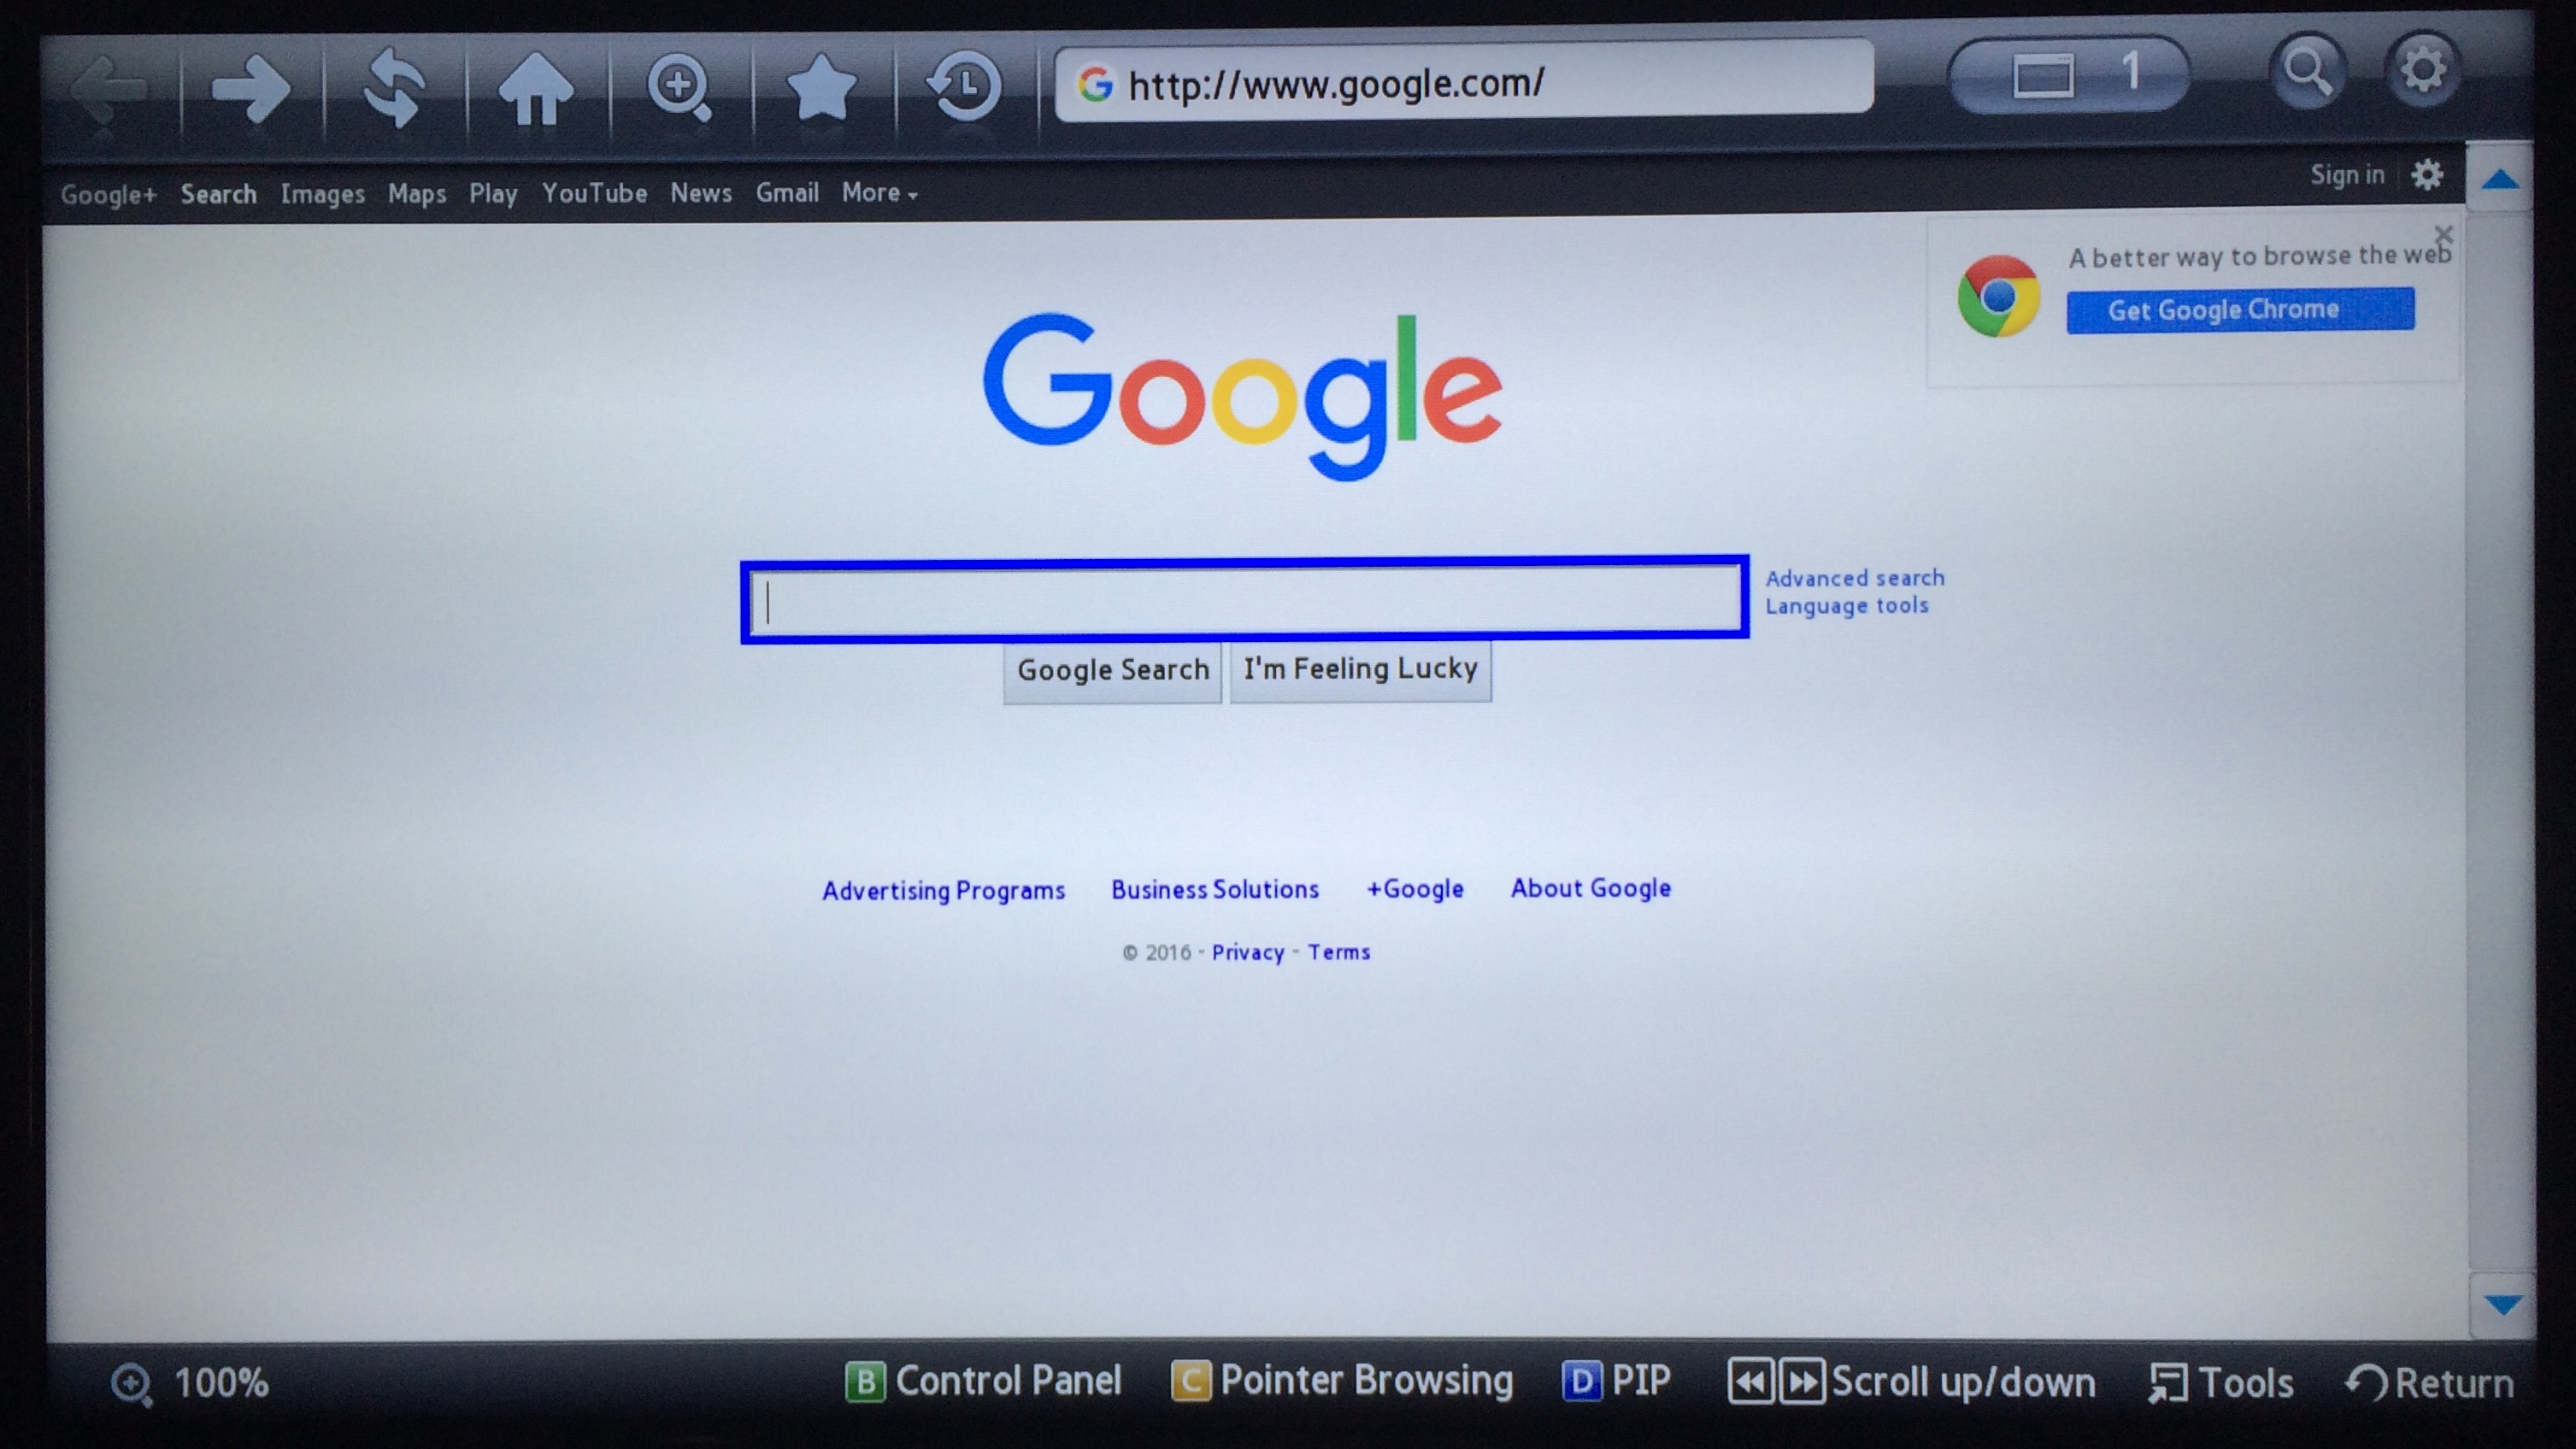
\includegraphics[height=50.5mm]{images/Browser.jpg}
	 \caption{Przeglądarka internetowa wbudowana w telewizor.}
\end{figure}


Środowisko internetowe gwarantuje nie tylko większą ilość użytkowników, lecz także mniejsze koszty uruchomieniowe danej aplikacji po stronie klienta. Aplikacje internetowe nie wymagają żadnego dodatkowego oprogramowania, ponieważ większość dzisiejszych urządzeń ma już je wbudowane. Dodatkowo są one uruchamiane na zewnętrznym serwerze co powoduje, iż obciążenie obliczeniowe aplikacji jest przenoszone na dostawcę usługi, a nie na użytkownika. 

Dzięki temu klient nie ponosi większych kosztów wynikających z użycia serwisu. Nie musi wymieniać sprzętu, instalować sterowników, pobierać aktualizacji. 

%bo się nie mieści kurka wodna
\newpage
\section{Cel aplikacji}
W niniejszej pracy został ukazany projekt aplikacji internetowej, której zadaniem jest umożliwienie nauki wybranych słówek danego języka obcego za pomocą wirtualnych fiszek, które będą prezentowane użytkownikowi w nieregularnych odstępach czasowych obliczanych na podstawie poprawności udzielonych odpowiedzi. Program podczas odpytywania użytkownika o dane słowo używa obrazów powiązanych z danym słowem. Ważnym założeniem aplikacji w trakcie procesu nauczania było jak najmniejsze wykorzystanie innego języka niż nauczany. 

%Zadaniem aplikacji jest umożliwienie nauki wybranych słówek danego języka obcego z pomocą wirtualnych fiszek, które będą prezentowane użytkownikowi w nieregularnych odstępach czasowych obliczanych na podstawie poprawności udzielonych odpowiedzi.
%Program powinien umożliwiać:
%\begin{itemize}
%	\item Dodawanie, modyfikowanie i usuwanie fiszek.
%	\item 
%\end{itemize}


%Program został stworzony w języku C\# z użyciem frameworka ASP.NET MVC. Wszystkie dane są przechowywane na serwerze Microsoft SQL. Po stronie klienta użyto języka HTML wraz z arkuszami styli stworzonymi w oparciu o język SASS. Wszystkie skrypty napisano w języku Scala, który jest potem kompilowany przez narzędzie Scala.js do 